\chapter{
Modeling Spatial Variation in Density
}
\markboth{Spatial Variation in Density}{}
\label{chapt.state-space}


\section{Homogeneous point process revisited}

\begin{figure}
\centering

\label{state-space.fig.homo}
\end{figure}

\begin{comment}
 
\begin{table}
  \centering
 
  \begin{tabular}{lccc}
    \hline
   
    \hline

    \hline
  \end{tabular}
  \label{state-space.tab.homo}
\end{table}
\end{comment}


\section{Inhomogeneous point processes}

\begin{equation}
  \label{state-space.eq.loglin}
\end{equation}

\begin{equation}
\label{state-space.eq.EN}
\end{equation}

\begin{equation}
  \label{state-space.eq.uprior}
\end{equation}

\begin{equation}
\label{state-space.eq.pdf.hetero}
\end{equation}

\begin{equation}
\label{state-space.eq.pdf.hetero.d}
\end{equation}

\begin{equation}
\label{state-space.eq.psimu}
\end{equation}

\begin{gather*}
\end{gather*}


\section{Observed Point Processes}

\begin{figure}
\centering
\label{state-space.fig.hetero}
\end{figure}

\section{Fitting inhomogeneous point process SCR models}

\subsection{Continuous space}

\begin{figure}
  \centering
   \label{state-space.fig.fm1post}
\end{figure}

\begin{table}
\centering
\begin{tabular}{lrrrr}
\hline

\hline

\hline
\end{tabular}
\label{state-space.tab.simIPP}
\end{table}

\subsection{Discrete space}
\label{modeling.sec.discrete}


\begin{figure}[ht]
\centering

\label{state-space.fig.discrete}
\end{figure}

\begin{panel}%[h!]
\centering
\rule[0.15in]{\textwidth}{.03in}
\begin{small}
\begin{verbatim}
model{
sigma ~ dunif(0, 20)
lam0 ~ dunif(0, 5)
beta0 ~ dunif(-10, 10)
beta1 ~ dunif(-10, 10)
for(j in 1:nPix) {
  mu[j] <- exp(beta0 + beta1*CANHT[j])*pixArea
  probs[j] <- mu[j]/EN
}
EN <- sum(mu[]) # Expected value of N, E[N]
psi <- EN/M
for(i in 1:M) {
  w[i] ~ dbern(psi)
  s[i] ~ dcat(probs[])
  x0g[i] <- Sgrid[s[i],1]
  y0g[i] <- Sgrid[s[i],2]
  for(j in 1:ntraps) {
    dist[i,j] <- sqrt(pow(x0g[i]-traps[j,1],2) + pow(y0g[i]-traps[j,2],2))
    lambda[i,j] <- lam0*exp(-dist[i,j]*dist[i,j]/(2*sigma*sigma)) * w[i]
    y[i,j] ~ dpois(lambda[i,j])
    }
  }
N <- sum(w[]) # Realized value of N
}
\end{verbatim}
\end{small}
\rule[0.15in]{\textwidth}{.03in}
\caption{\bugs~code for fitting inhomogeneous point process model in
  discrete space.}
\label{state-space.panel1}
\end{panel}

\begin{table}%[h!]
\centering
\caption{Comparison of \secr~and \jags~results. Point estimates from
  the Bayesian analysis are posterior means. Intervals are lower and
  upper 95\% CIs.}
\begin{tabular}{lrlrrrr}
\hline
Parameter 	& Truth 	& Software 	& Mean 	& SD 	& 2.5\% & 97.5\% \\
\hline
 $\lambda_0$ 	&  1.00 	& \textbf{JAGS} 	&  1.04 	& 0.087 	&  0.88 	&  1.22 \\
  	&  1.00 	& \texttt{secr} 	&  1.08 	& 0.089 	&  0.92 	&  1.27 \\
 $\sigma$ 	& 10.00 	& \textbf{JAGS} 	& 10.16 	& 0.373 	&  9.46 	& 10.94 \\
  	& 10.00 	& \texttt{secr} 	&  9.84 	& 0.350 	&  9.18 	& 10.55 \\
 $\beta_1$ 	&  1.00 	& \textbf{JAGS} 	&  1.20 	& 0.350 	&  0.50 	&  1.88 \\
  	&  1.00 	& \texttt{secr} 	&  1.09 	& 0.316 	&  0.47 	&  1.71 \\
 $N$ 	& 30.00 	& \textbf{JAGS} 	& 26.63 	& 2.585 	& 23.00 	& 33.00 \\
  	& 30.00 	& \texttt{secr} 	& 28.19 	& 3.037 	& 24.49 	& 37.39 \\
 $\mathbb{E}[N]$ 	& 32.30 	& \textbf{JAGS} 	& 26.39 	& 5.048 	& 17.25 	& 36.96 \\
  	& 32.30 	& \texttt{secr} 	& 28.19 	& 6.117 	& 18.52 	& 42.93 \\
\hline
\end{tabular}
\label{state-space.tab.jagsVsecr}
\end{table}


\section{Ecological Distance and Density Covariates}

\begin{figure}[ht]
\centering
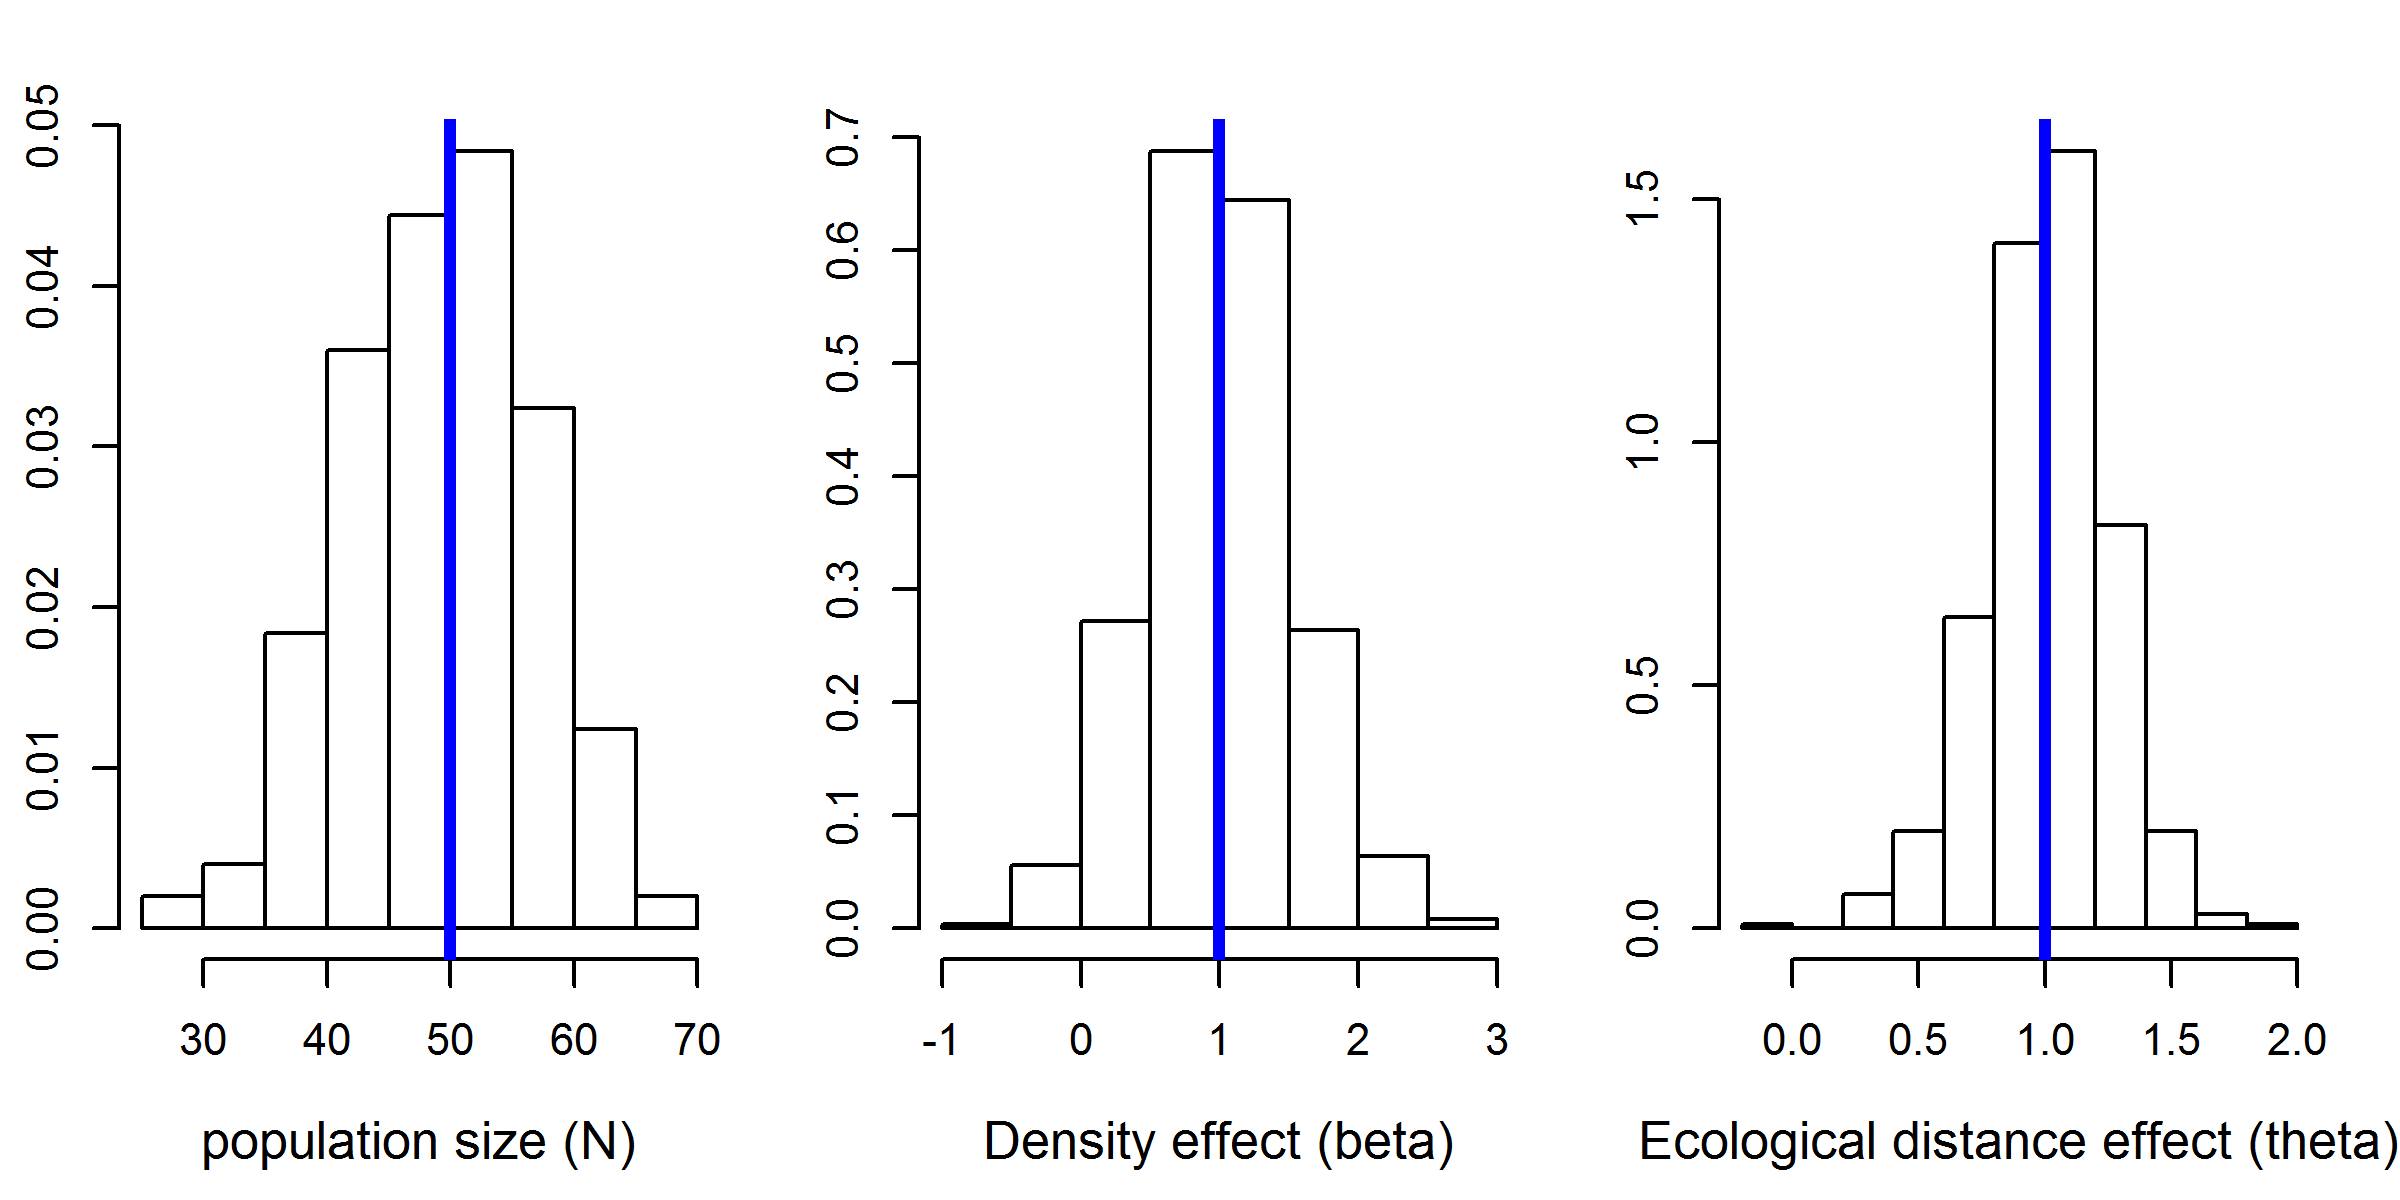
\includegraphics[width=4in,height=2in]{Ch11-Statespace/figs/scrDEDsim}
\caption{Histograms of parameter estimates from 500 simulations under
  the model in which both density and ecological distance are affected
by the same covariate, canopy height. The vertical lines indicate the
data-generating value.}
\label{ch9.fig.sim}
\end{figure}


\section{The Jaguar Data}

\begin{figure}%[ht]
\centering
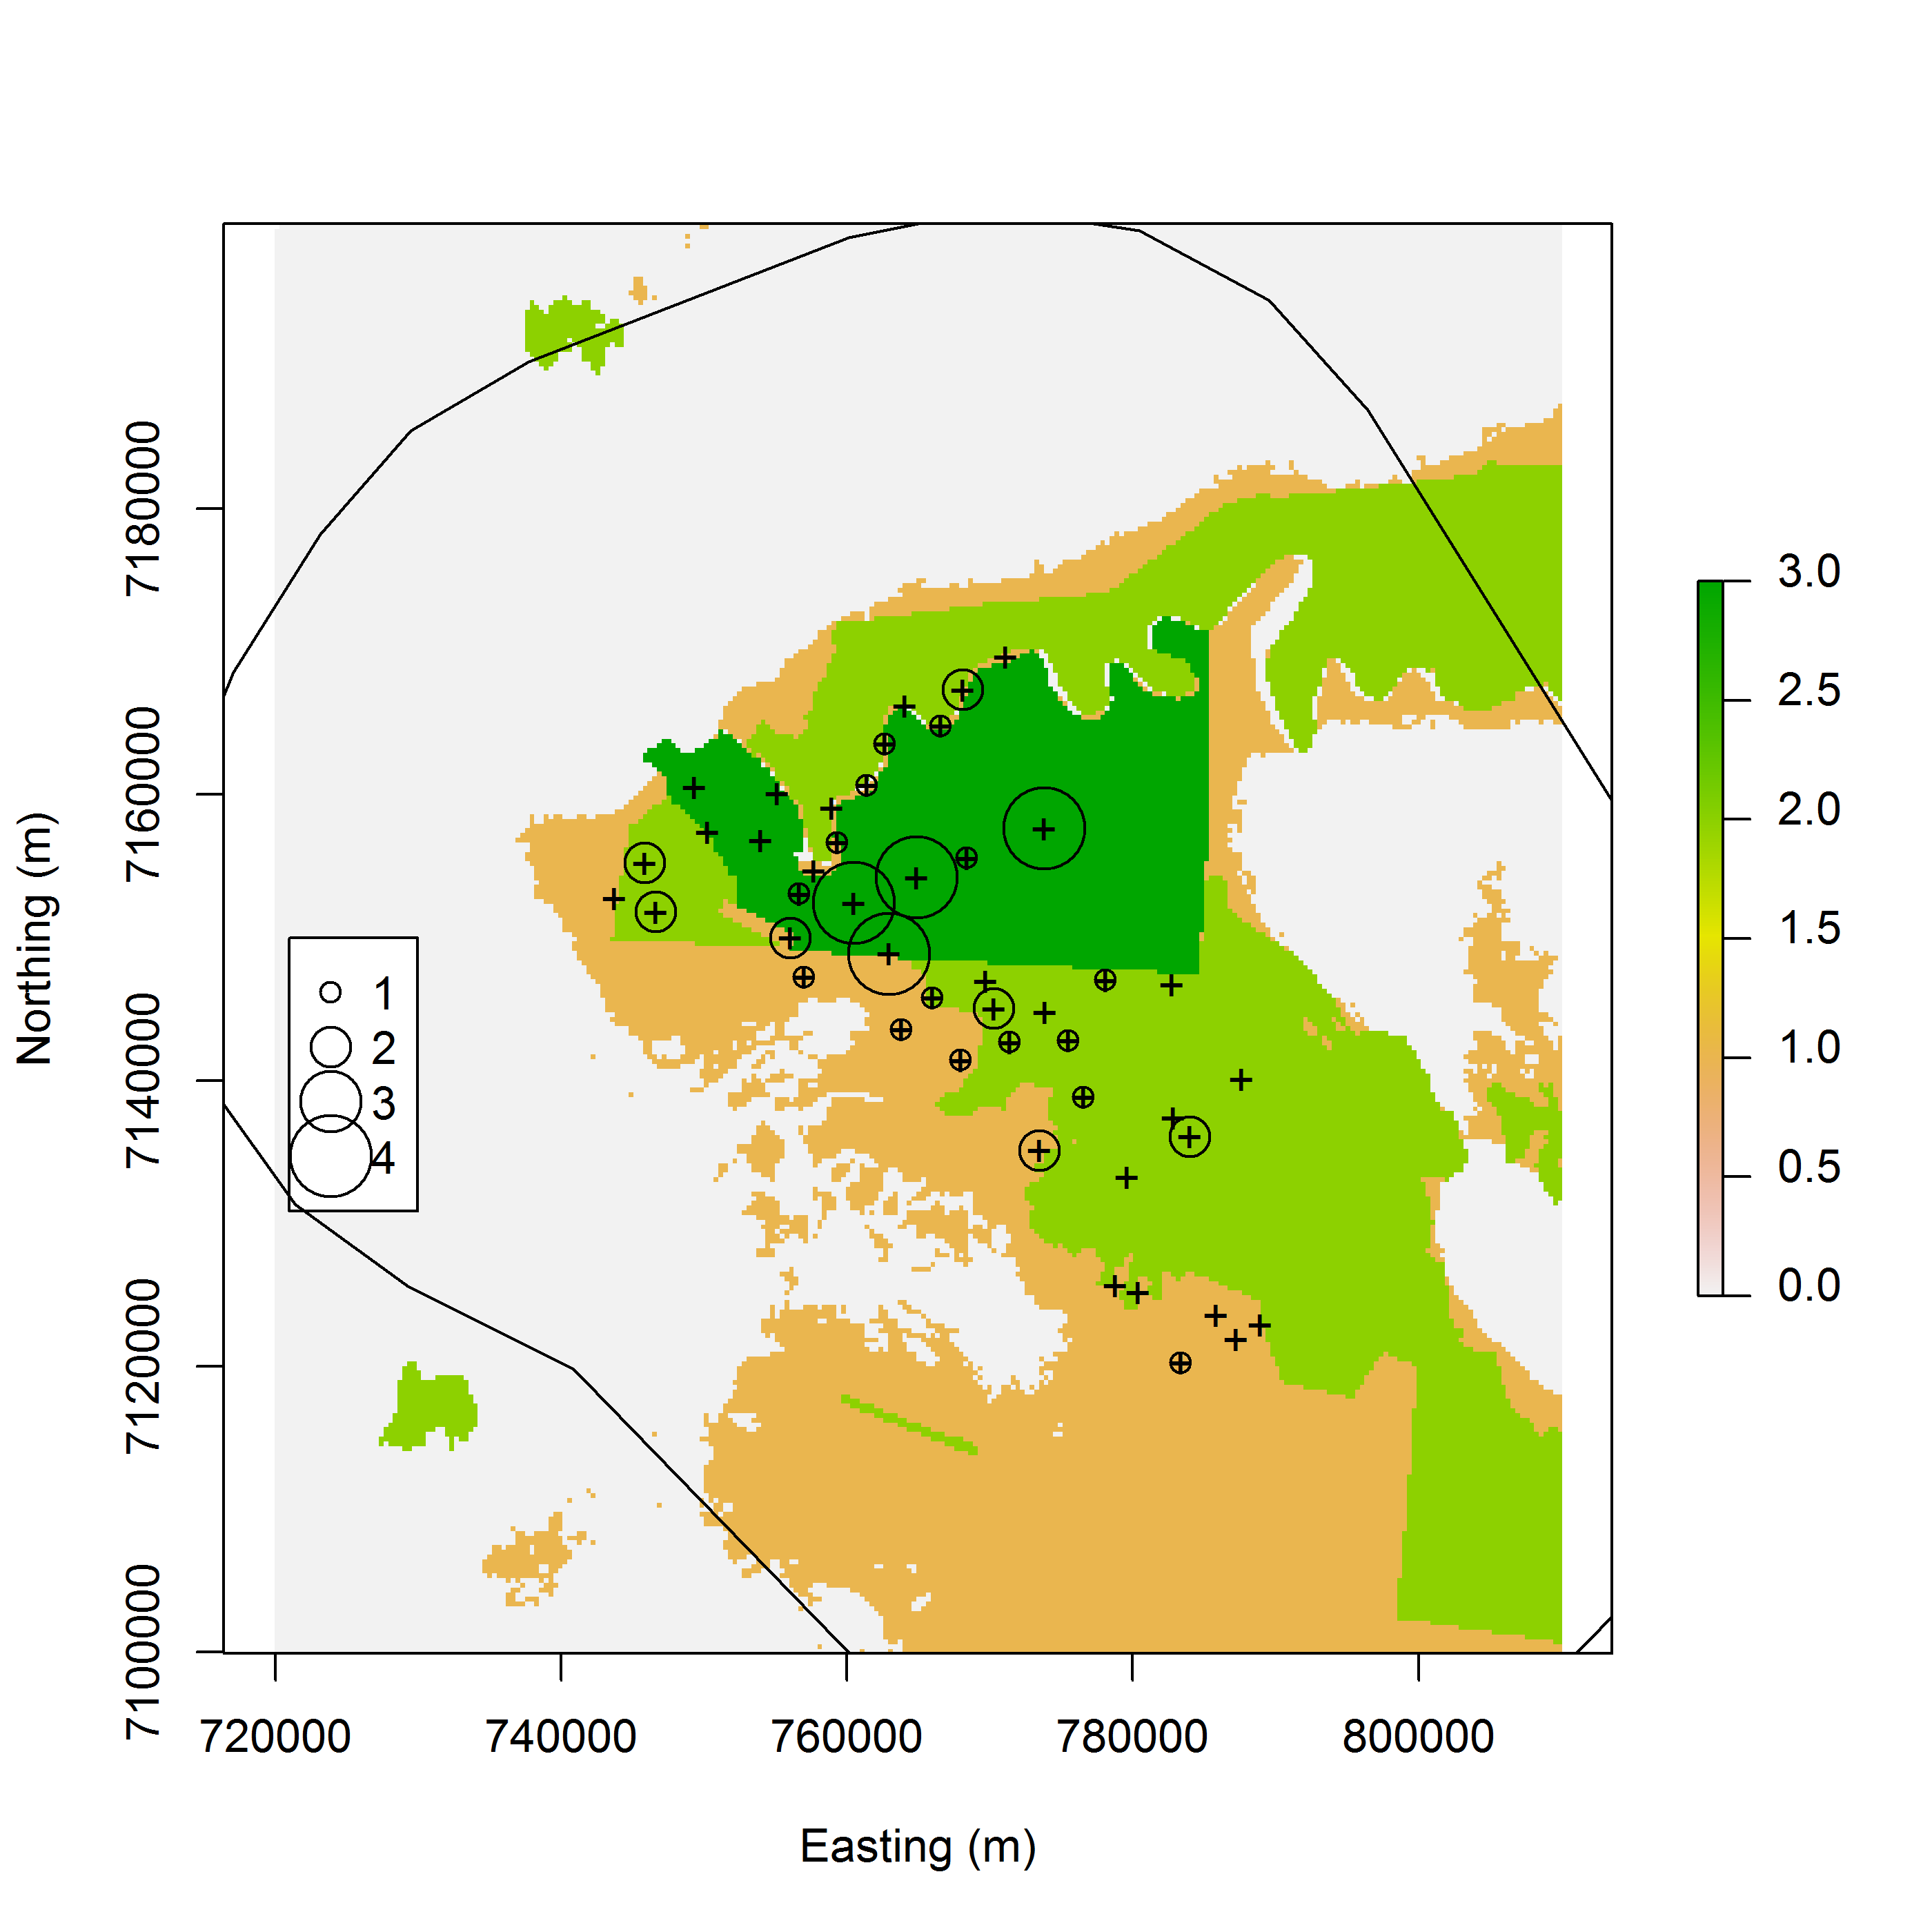
\includegraphics[width=0.6\textwidth]{Ch11-Statespace/figs/jaguarCountMap}
\label{state-space.fig.jaguarCts}
\caption{Jaguar detections at 46 camera trap stations. The three levels of
  protection status are no protection (beige), some protection (light
  green), and Iguaz\'{u} National Park (dark green). Non-habitat
  (soybean monocultures) is shown in gray. }
\end{figure}

\begin{table}
\centering
\caption{Summaries of posterior distributions from the model of jaguar
  density. $\sigma$ is the scale parameter of
  the half-normal detection function. $\lambda_0$ is base-line encounter rate. $\beta_1$ is the
  effect of protection status on jaguar density. $\rho$ is the
  sex-ratio.  $N$ is population size. The last three parameters are the density estimates
  (jaguars/100km$^2$) for the three levels of protection.}
\begin{tabular}{lrrrr}
\hline
& Mean & SD & 2.5\% & 97.5\% \\
\hline
 $\sigma_\text{female}$ 	& 5434.886 	& 883.7433 	& 4093.6069 	& 7549.062 \\
 $\sigma_\text{male}$ 	& 6208.341 	& 822.6217 	& 4881.4060 	& 8093.759 \\
 $\lambda_0$ 	&    0.013 	&   0.0036 	&    0.0068 	&    0.021 \\
 $\beta_0$ 	&   -4.667 	&   0.2866 	&   -5.2527 	&   -4.093 \\
 $\beta_1$ 	&    0.196 	&   0.3672 	&   -0.5179 	&    0.961 \\
 $\rho$ 	&    0.541 	&   0.0551 	&    0.4286 	&    0.644 \\
 $N$ 	        &   36.428 	&   9.6986 	&   23.0000 	&   61.000 \\
 $D_\text{low}$ 	&    0.921 	&   0.3851 	&    0.3789 	&    1.894 \\
 $D_\text{med}$ 	&    0.775 	&   0.3006 	&    0.2653 	&    1.503 \\
 $D_\text{high}$ &    1.444 	&   0.3325 	&    0.8791 	&    2.110 \\
 \hline
\end{tabular}
\label{state-space.tab.jagposts}
\end{table}

\begin{figure}%[ht]
\centering
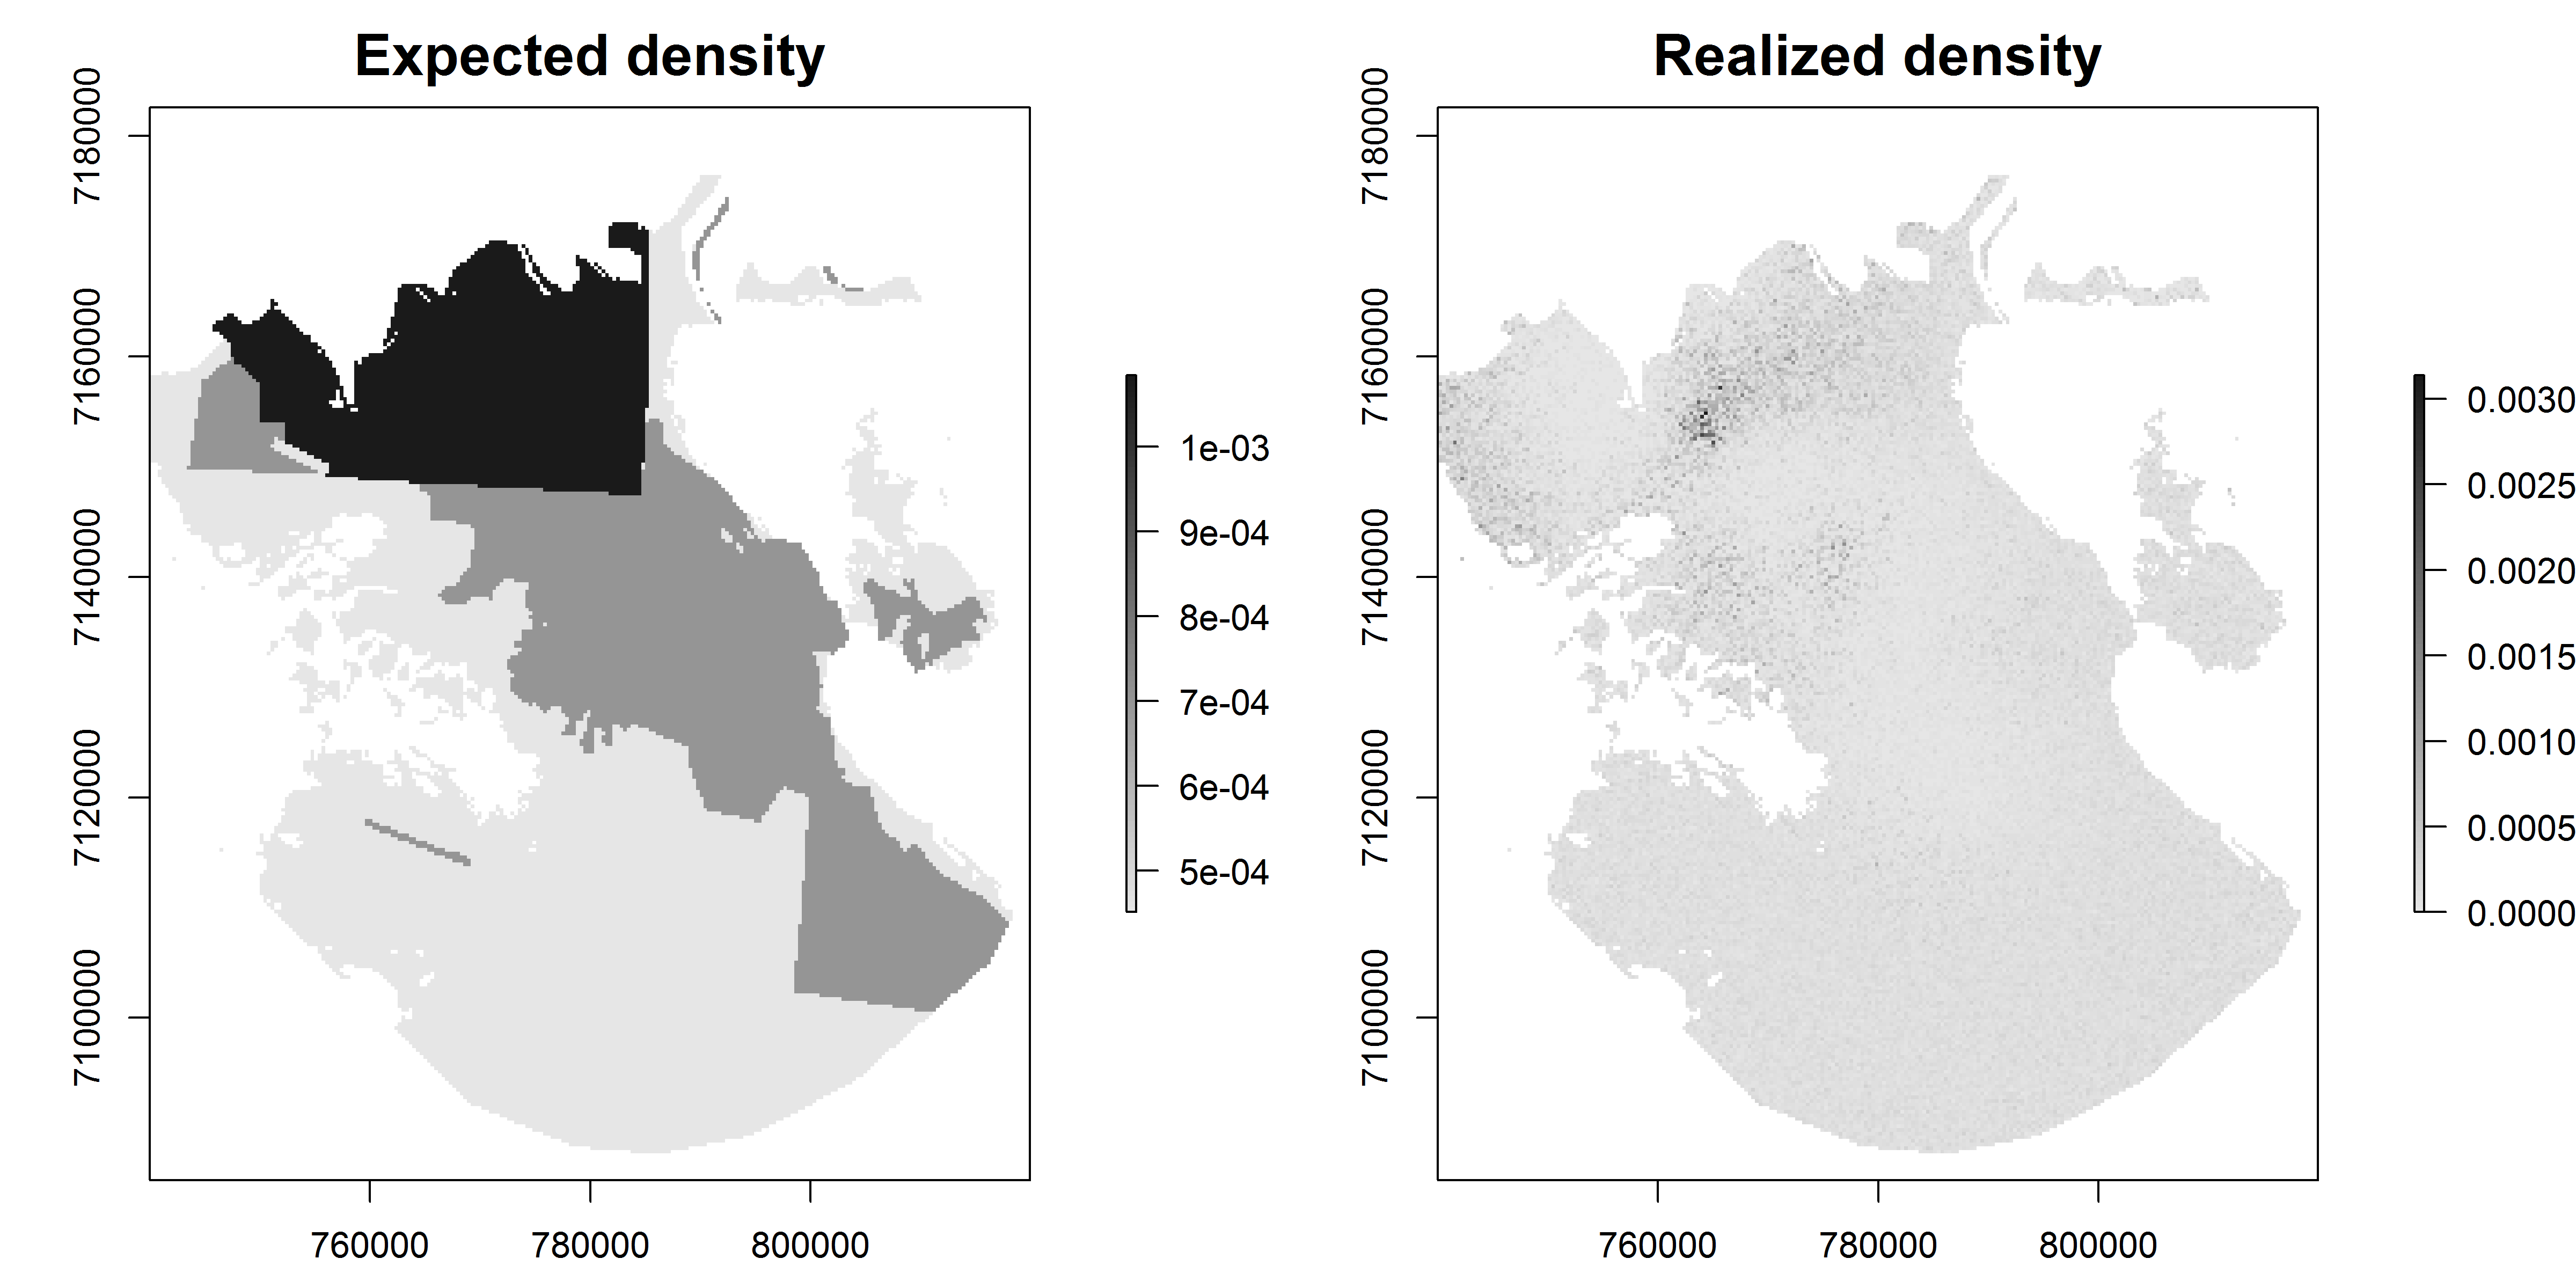
\includegraphics[width=\textwidth]{Ch11-Statespace/figs/reD}
\label{state-space.fig.Dsurface}
\caption{Estimated density surfaces from the analysis of the jaguar data.}
\end{figure}


\section{Summary and Outlook}
